\subsection{Estudos de Regressão}

Ao montarmos a visualização dos tempos entre chegadas ao longo do tempo percebemos que havia tendência nos dados. Para isso, primeiro, calculamos todos os intervalos entre a chegada das chamadas, subtraindo o horário de recebimento de uma chamada subsequente pelo da anterior, isto é:

$$Intervalo_{chegada}(c_n) = t_n - t_{n-1}$$ 

\begin{itemize}
    \item $c_n$ é a chamada de número $n$
    \item $t_n$ é o tempo de recebimento da chamada $n$
    \item $t_{n-1}$ é o tempo de recebimento da chamada $n-1$
\end{itemize}

Depois, as chamadas foram classificadas por dia, e, assim, calculado o intervalo de chegada médio diário delas. O principal intuito desta etapa é facilitar a visualização da evolução desse parâmetro ao longo do tempo. O gráfico obtido por essa operação está na Figura \ref*{fig: arrivals-tempo}.

A partir dessa percepção, são então propostos alguns estudos de regressão mais particulares para representar a tendência dos dados. Um usando "Ordinary Least Squares"\;e uma regressão exponencial.  

\subsubsection{Ordinary Least Squares (Regressão linear)}

Utilizando a biblioteca Statsmodel do Python foi realizado o estudo de regressão. A Equação Obtida foi: $$intervalos(t) = -0,4933 \cdot t + 252,6629$$ O resumo da regressão é mostrado na Figura \ref*{fig: sum_OLS} e o plot na Figura \ref*{fig: plot_OLS}.

\begin{figure}[H]
    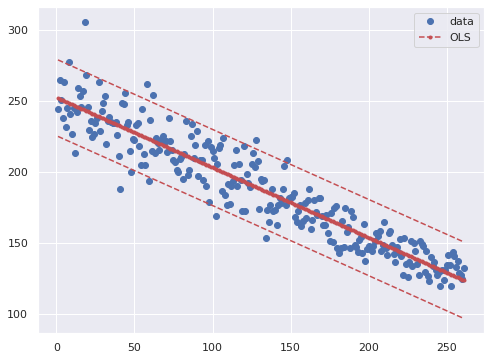
\includegraphics[scale=0.9]{analise-de-dados/regressao/regressao_OLS.png}
    \caption{Regressão Linear para os tempos de espera}
    \label{fig: plot_OLS}
\end{figure}

\begin{figure}[H]
    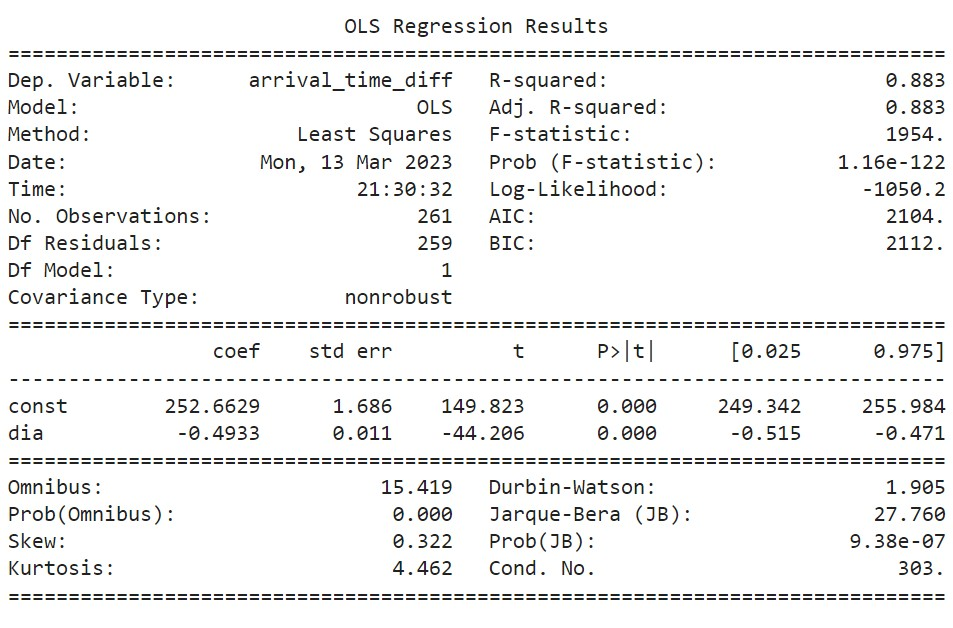
\includegraphics[scale = 0.85]{analise-de-dados/regressao/OLS_summary.jpg}
    \caption{Resumo da regressão}
    \label{fig: sum_OLS}
\end{figure}

Temos que os valores p são menores que o nível de significância adotado, e, portanto, o modelo de regressão existe. Entretanto, para os dias em que $t > 512$ o tempo de chegada das chamadas seria negativo, o que levanta questões sobre se este método de regressão é aplicável para modelar o tempo entre as chamadas.

\subsubsection{OLS exponencial}

De maneira semelhante ao primeiro estudo, este também foi feito utilizando a biblioteca statsmodel. Entretanto, ao invés dos parâmetros para a regressão terem sido adicionados como são ao modelo, ele foi construído usando: $$ln(y) = ln(b) + a \cdot x$$

Dessa maneira, a equação obtida para representar os dados foi:
$$intervalos(t) = 260,9424 \cdot e^{-0,0027x} $$

O resumo e o gráfico da regressão estão nas Figuras \ref*{fig: sum_Expo_OLS} e \ref*{fig: plot_Expo_OLS}, respectivamente.
\begin{figure}[H]
    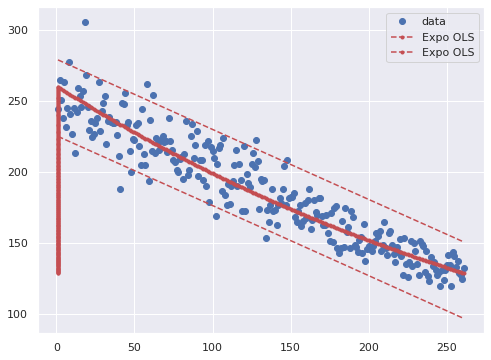
\includegraphics{analise-de-dados/regressao/regressao_EXPO.png}
    \caption{Regressão Exponencial para os tempos de espera}
    \label{fig: plot_Expo_OLS}
\end{figure}

\begin{figure}[H]
    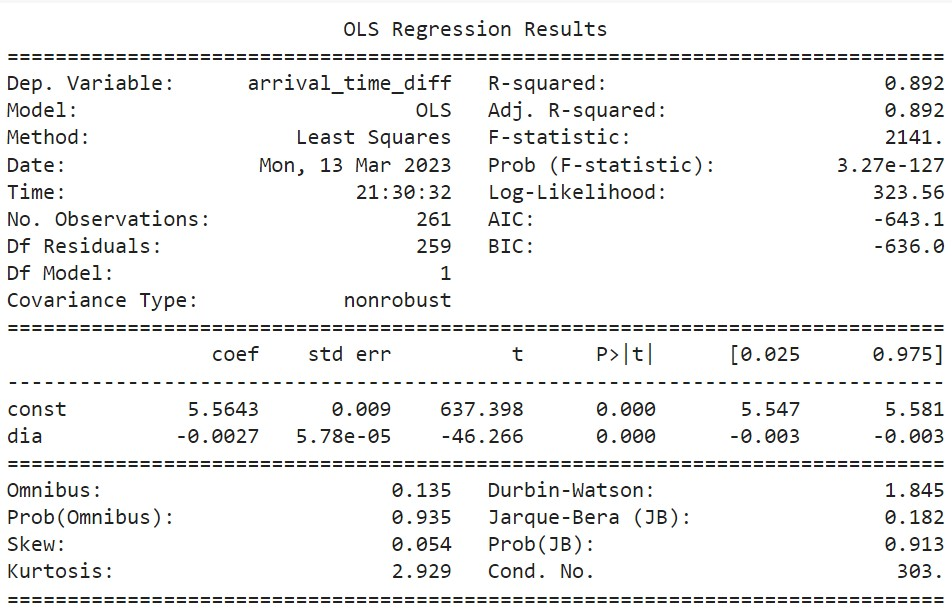
\includegraphics[scale = 0.85]{analise-de-dados/regressao/EXPO_OLS_Summary.jpg}
    \caption{Resumo da regressão}
    \label{fig: sum_Expo_OLS}
\end{figure}

Para este caso, a explicabilidade do modelo aumentou e o problema da obtenção de intervalos negativos com a regressão linear deixou de existir. Como os valores $p$ seguem menores do que 0, o modelo existe e pode ser usado.
